\documentclass{bschlangaul-aufgabe}
\bLadePakete{uml,java}
\begin{document}
\bAufgabenMetadaten{
  Titel = {1 Firmenstruktur},
  Thematik = {Firmenstruktur},
  Referenz = 46116-2011-F.T1-TA2-A1,
  RelativerPfad = Staatsexamen/46116/2011/03/Thema-1/Teilaufgabe-2/Aufgabe-1.tex,
  ZitatSchluessel = examen:46116:2011:03,
  BearbeitungsStand = mit Lösung,
  Korrektheit = unbekannt,
  Ueberprueft = {unbekannt},
  Stichwoerter = {Einfach-verkettete Liste, Objektdiagramm},
  EinzelpruefungsNr = 46116,
  Jahr = 2011,
  Monat = 03,
  ThemaNr = 1,
  TeilaufgabeNr = 2,
  AufgabeNr = 1,
}

\let\j=\bJavaCode

\section{Firmenstruktur
\index{Einfach-verkettete Liste}
\footcite{examen:46116:2011:03}}

\begin{center}
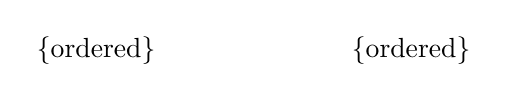
\begin{tikzpicture}
\node (ordered1) at (2,3) {\{ordered\}};
\node (ordered2) at (6,3) {\{ordered\}};

\umlclass[x=0]{Firma}{}{+ addAbteilung(name: String)\\+ erzeugelDs()}
\umlclass[x=4.5]{Abteilung}{+ name: String}{}
\umlclass[x=8]{Angestellter}{+ id: int}{}
\umlassoc[arg1=+ firma,mult1=1,pos1=0.7]{ordered1}{Firma}
\umlassoc[arg1=+ abteilungen,mult1=*,pos1=0.5]{ordered1}{Abteilung}
\umlassoc[arg1=+ abteilung,mult1=1,pos1=0.7]{ordered2}{Abteilung}
\umlassoc[arg1=+ angestellte,mult1=*,pos1=0.7]{ordered2}{Angestellter}
\end{tikzpicture}
\end{center}

\noindent
Eine Firma besteht aus \j{null} oder mehr Abteilungen, von
denen jede \j{null} oder mehr Angestellte hat. Da sowohl die
Abteilungen als auch deren Angestellten geordnet sind, sind Angestellte
insgesamt geordnet. Sie haben durchgehende, ganzzahlige IDs, die bei 1
beginnen.

\begin{enumerate}

%%
% a)
%%

\item Erstellen Sie exemplarisch ein Objektdiagramm: Stellen Sie eine
Firma mit dem Instanznamen \j{f} und den zwei Abteilungen
„Produktion“ (Name \j{p}) und „Marketing“ (Name \j{m})
dar. Die Produktion hat zwei Angestellte, Marketing hat einen
Angestellten. Die Angestellten haben die Namen \j{a1},
\j{a2}, und \j{a3}.
\index{Objektdiagramm}

\begin{bAntwort}
Die Instanzbezeichnung müsste noch unterstrichen werden. Das geht aber
leider mit TikZ-UML nicht.
\begin{center}
\begin{tikzpicture}

\umlclass[x=0,y=0]{f : Firma}{}{}

\umlclass[x=0,y=-2]{p : Abteilung}{name = “Produktion”}{}
\umlclass[x=4,y=-2]{m : Abteilung}{name = “Marketing”}{}

\umlclass[x=0,y=-4,name=a1]{a1 : Angestellter}{id = “1”}{}
\umlclass[x=3,y=-4]{a2 : Angestellter}{id = “2”}{}
\umlclass[x=6,y=-4]{a3 : Angestellter}{id = “3”}{}

\umluniassoc{f : Firma}{p : Abteilung}
\umluniassoc{p : Abteilung}{m : Abteilung}
\umluniassoc{p : Abteilung}{a1 : Angestellter}
\umluniassoc{a1 : Angestellter}{a2 : Angestellter}

\umluniassoc{m : Abteilung}{a3 : Angestellter}

\end{tikzpicture}
\end{center}
\end{bAntwort}

%%
% b)
%%

\item Implementieren Sie das Klassendiagramm in Java oder in einer
anderen geeigneten objektorientierten Programmiersprache Ihrer Wahl.
Beachten Sie, dass die Assoziationen bidirektional und geordnet sind.
Die beiden Methoden der Klasse \j{Firma} sollen dabei folgendes
Verhalten haben:

Die Methode \j{erzeugeIDs} sorgt dafür, dass die IDs wieder
korrekt zugewiesen sind. Die alten IDs können beliebig geändert werden,
solange das Endergebnis wieder den obenstehenden Kriterien genügt.

\begin{bAntwort}
\bJavaExamen[firstline=3]{46116}{2011}{03}{Firma}
\bJavaExamen[firstline=3]{46116}{2011}{03}{Abteilung}
\bJavaExamen[firstline=3]{46116}{2011}{03}{Angestellter}
\end{bAntwort}

%%
% c)
%%

\item Angestellte sollen in Manager und einfache Angestellte unterteilt
werden. Zeichnen Sie ein Klassendiagramm mit der Oberklasse
\j{Angestellter} und den zwei Unterklassen \j{Manager}
und \j{EinfacherAngestellter}. Die Klasse
\j{Angestellter} soll nicht instantiierbar sein und erzwingen,
dass die Methode \j{getPosition()} (öffentlich, ohne Argumente,
Rückgabewert \j{String}) von allen konkreten Unterklassen
implementiert wird. \j{Manager} und
\j{EinfacherAngestellter} sollen instantiierbar sein.

\begin{bAntwort}
\begin{center}
\begin{tikzpicture}

\umlclass[x=0,y=0,type=abstract]{Angestellter}{\textit{+ getPosition(): String}}{}
\umlclass[x=-3,y=-3]{Manager}{
+ Manager()\\
+ getPosition(): String}{}

\umlclass[x=3,y=-3]{EinfacherAngestellter}{
+ EinfacherAngestellter()\\
+ getPosition(): String}{}

\umlVHVinherit{Manager}{Angestellter}
\umlVHVinherit{EinfacherAngestellter}{Angestellter}
\end{tikzpicture}
\end{center}
\end{bAntwort}

%%
% d)
%%

\item Wie lautet der Fachbegriff dafür, dass eine Methode in einer
Klasse und in deren Unterklassen dieselbe Signatur hat, aber in den
Unterklassen unterschiedlich implementiert ist?

\begin{bAntwort}
Abstrakte Methode
\end{bAntwort}
\end{enumerate}

\end{document}
